\section{Results}
\label{sec:results}
All numbers are means over the \NumTest\ test mixtures with bootstrap 95\%
CIs, unless marked \emph{held-out} (\NumHeldout\ mixtures, unseen head and
noise). Table~\ref{tab:main} lists every cell.

\begin{figure*}[t]
\centering
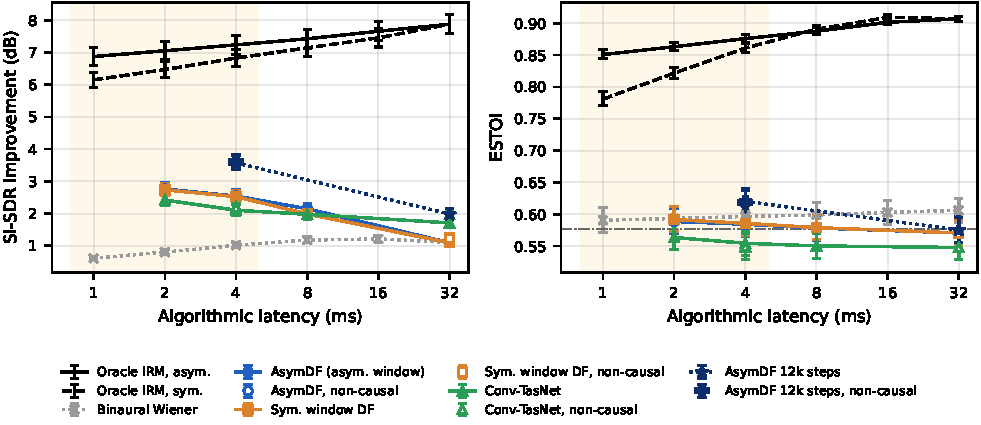
\includegraphics[width=\textwidth]{figures/quality_vs_latency.pdf}
\caption{Quality against algorithmic latency. The shaded band is the
hearing-aid budget ($\le$5\,ms). Solid markers are causal models (2k
steps); hollow markers are non-causal twins; stars are the 12k-step AsymDF
runs. The symmetric-window family coincides with AsymDF at 32\,ms, where
the two windows are identical. Black lines are oracle ratio masks.}
\label{fig:quality}
\end{figure*}

\subsection{What the window costs: the oracle bound}
With an asymmetric window, the ideal ratio mask gains \OracleEarAsymOnems\,dB
SI-SDRi at 1\,ms and \OracleEarAsymThreeTwoms\,dB at 32\,ms
(Fig.~\ref{fig:quality}). Going from 32\,ms down to 1\,ms therefore costs
about 1\,dB even for a perfect mask. A symmetric window loses more
(\OracleEarSymOnems\,dB at 1\,ms), and the asymmetric analysis recovers
\OracleAsymGainOnems\,dB of it at 1\,ms and \OracleAsymGainFourms\,dB at
4\,ms. The effect is clearer in intelligibility: oracle ESTOI at 1\,ms is
\OracleEarAsymEstoiOnems\ with the asymmetric window against
\OracleEarSymEstoiOnems\ with the symmetric one. Frequency resolution is a
real cost, but a small and mostly recoverable one.

\subsection{What the future buys: almost nothing}
At 4\,ms, the non-causal AsymDF, which sees the whole utterance, scores
\stftasymFourmsearnc\,dB against \stftasymFourmsear\,dB for its causal
twin. After 12k steps the scores are \stftasymFourmsearnclong\ vs.\
\stftasymFourmsearlong\,dB (Fig.~\ref{fig:gap}). Conv-TasNet shows the same
at 4\,ms (\tasnetFourmsearnc\ vs.\ \tasnetFourmsear\,dB) and gains at most
a few tenths of a dB at 32\,ms (\tasnetThreeTwomsearnc\ vs.\
\tasnetThreeTwomsear\,dB). Explicit lookahead tells the same story
(Fig.~\ref{fig:lookahead}). At a fixed 8\,ms budget, spending latency on
lookahead looks better (\LookaheadZeroSdr\,dB with $D{=}0$ vs.\
\LookaheadBestSdr\,dB with $D{=}\LookaheadBestD$), but those runs also have
smaller hops. At a \emph{matched} hop, lookahead changes SI-SDRi by
\LookaheadGainTwohopTwoms\,dB (+4\,ms of future, 95\% CI
[\LookaheadGainTwohopTwomsLo, \LookaheadGainTwohopTwomsHi]) and
\LookaheadGainSixhopOnems\,dB (+6\,ms, CI
[\LookaheadGainSixhopOnemsLo, \LookaheadGainSixhopOnemsHi]). The future is
not what limits these models.

\begin{figure}[t]
\centering
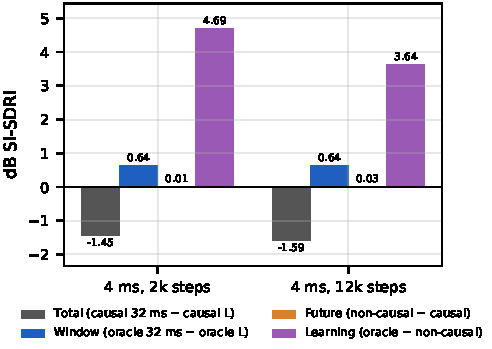
\includegraphics[width=\columnwidth]{figures/gap_decomposition.pdf}
\caption{Where the 4\,ms causal AsymDF stands relative to 32\,ms, at two
training budgets. The window cost is an oracle quantity; the future and
learning terms come from the trained non-causal twin.}
\label{fig:gap}
\end{figure}

\subsection{What learning costs: everything else}
The gap that remains is learning. At 4\,ms the oracle exceeds the
non-causal model by \GapLearningFourms\,dB after 2k steps and by
\LongGapLearningFourms\,dB after 12k (Fig.~\ref{fig:gap}), against
\GapResolutionFourms\,dB for the window and \LongGapFutureFourms\,dB for
the future. The asymmetric window's oracle advantage does not show up in
the trained models either: the symmetric twin is within 0.2\,dB at every
latency (\stftsymTwomsear\ vs.\ \stftasymTwomsear\,dB at 2\,ms). At this
model size and training budget, a 4\,ms device would gain more from a
better-trained network than from any amount of latency.

\paragraph{Shorter latency trains faster.}
At equal steps, quality \emph{falls} with latency in every family
(paired Wilcoxon, AsymDF 2$\to$4\,ms $\Delta$=\WilstftasymTwotoFourdiff\,dB,
$p$=\WilstftasymTwotoFourp; 8$\to$32\,ms
$\Delta$=\WilstftasymEighttoThreeTwodiff\,dB,
$p$=\WilstftasymEighttoThreeTwop). This is the opposite of the oracle
trend. A 1\,ms hop gives 16$\times$ more supervised frames per step than a
16\,ms hop, so equal steps are not equal training. Six times more steps
did not close it either: the 32\,ms model reaches
\stftasymThreeTwomsearlong\,dB and the 4\,ms model \stftasymFourmsearlong\,dB.
The pre-registered gap criterion (4\,ms within 1\,dB of 32\,ms) is
therefore met (gap \HypGapPrimary\,dB, \HypGapSource\ budget), but for the
wrong reason, and we do not count it as support.

\begin{figure*}[t]
\centering
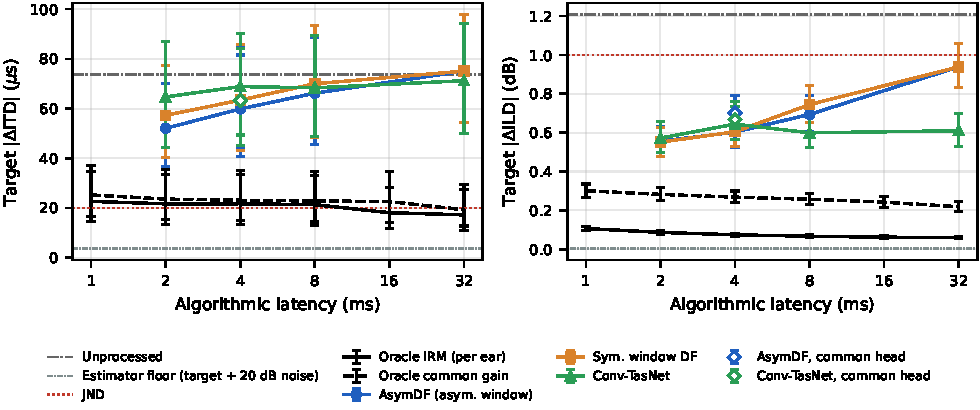
\includegraphics[width=\textwidth]{figures/cues_vs_latency.pdf}
\caption{Target interaural-cue errors against the clean binaural target.
Red: JND (20\,$\mu$s, 1\,dB). Grey dotted: the estimator's own floor
(target plus independent noise at 20\,dB SNR).}
\label{fig:cues}
\end{figure*}

\subsection{Interaural cues}
Level cues survive (Fig.~\ref{fig:cues}). Every causal model keeps the
target $|\Delta$ILD$|$ below the 1\,dB JND, down from \UnprocIld\,dB in
the mixture (\stftasymFourmsearlongIld\,dB for the 12k-step 4\,ms
AsymDF). Timing cues do not. No trained model gets $|\Delta$ITD$|$ near
20\,$\mu$s: the best is \stftasymFourmsearlongItd\,$\mu$s, against
\UnprocItd\,$\mu$s unprocessed. Even the oracle sits at
\OracleEarAsymItdFourms\,$\mu$s, while the estimator floor is only
\FloorItdTwoZerodB\,$\mu$s, so the oracle's error is real. Late
reverberation and noise left in low-frequency bins pull the broadband ITD.
The common-gain head does not fix this on the training head
(\stftasymFourmscommonItd\,$\mu$s), but it generalises best to the unseen
head: held-out SI-SDRi is \stftasymFourmscommonHeldout\,dB against
\stftasymFourmsearHeldout\,dB for the per-ear deep filter.

\begin{table*}[t]
\centering
\small
\begin{tabular}{llrrrrr}
\toprule
Model & $L$ & SI-SDRi & ESTOI & $|\Delta$ITD$|$ & $|\Delta$ILD$|$ & held-out \\
 & (ms) & (dB) & & ($\mu$s) & (dB) & SI-SDRi \\
\midrule
Unprocessed & -- & 0.00 & 0.577 & 73.8 & 1.21 & 0.00 \\
AsymDF & 2 & 2.76 & 0.589 & 52.1 & 0.56 & 0.52 \\
AsymDF & 4 & 2.54 & 0.584 & 59.9 & 0.60 & 0.44 \\
AsymDF (common head) & 4 & 2.24 & 0.577 & 63.4 & 0.70 & 1.58 \\
AsymDF (12k steps) & 4 & 3.57 & 0.620 & 47.8 & 0.36 & 1.00 \\
AsymDF (non-causal) & 4 & 2.55 & 0.584 & 63.8 & 0.58 & 0.53 \\
AsymDF (non-causal) (12k steps) & 4 & 3.60 & 0.618 & 47.0 & 0.36 & 0.93 \\
AsymDF & 8 & 2.15 & 0.578 & 66.2 & 0.69 & 0.49 \\
AsymDF & 32 & 1.09 & 0.571 & 75.1 & 0.94 & -0.61 \\
AsymDF (12k steps) & 32 & 1.98 & 0.575 & 69.3 & 0.73 & 0.31 \\
AsymDF (non-causal) & 32 & 1.23 & 0.570 & 73.2 & 0.91 & 0.05 \\
Sym. window DF & 2 & 2.73 & 0.592 & 57.3 & 0.55 & 0.93 \\
Sym. window DF & 4 & 2.52 & 0.586 & 63.4 & 0.60 & 0.79 \\
Sym. window DF & 8 & 1.99 & 0.579 & 70.0 & 0.74 & 0.55 \\
Conv-TasNet & 2 & 2.42 & 0.563 & 64.7 & 0.57 & 1.00 \\
Conv-TasNet & 4 & 2.10 & 0.554 & 68.8 & 0.64 & 1.10 \\
Conv-TasNet (common head) & 4 & 2.09 & 0.555 & 63.3 & 0.67 & 1.07 \\
Conv-TasNet (non-causal) & 4 & 2.20 & 0.549 & 61.6 & 0.59 & 1.05 \\
Conv-TasNet & 8 & 1.98 & 0.550 & 68.3 & 0.60 & 1.12 \\
Conv-TasNet & 32 & 1.71 & 0.548 & 71.2 & 0.61 & 0.46 \\
Conv-TasNet (non-causal) & 32 & 1.96 & 0.547 & 60.1 & 0.50 & 0.64 \\
\bottomrule
\end{tabular}

\caption{Test-set results for every cell (2k steps unless noted).
$|\Delta$ITD$|$ and $|\Delta$ILD$|$ are target-cue errors against the clean
early target. The last column is SI-SDRi on the held-out set (CIPIC head,
unseen noise environments and rooms).}
\label{tab:main}
\end{table*}

\subsection{Generalisation}
Every model loses most of its gain on the held-out set, for example
\stftasymFourmsearHeldout\,dB at 4\,ms (AsymDF) and
\tasnetFourmsearHeldout\,dB (Conv-TasNet), against
\stftasymFourmsear\ and \tasnetFourmsear\,dB on test. The per-ear deep
filter on the long asymmetric window transfers worst. The symmetric-window
filter (\stftsymFourmsearHeldout\,dB at 4\,ms), Conv-TasNet and the common
gain keep more. Fine per-ear spectral detail is what is most tied to one
head's HRTF, so a new head and new noise expose it first.

\begin{figure}[t]
\centering
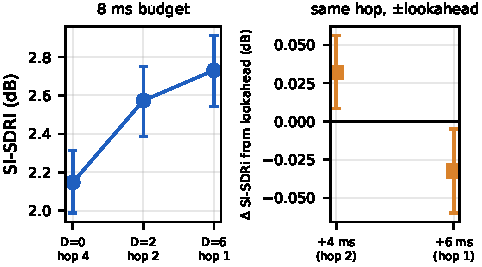
\includegraphics[width=\columnwidth]{figures/lookahead_split.pdf}
\caption{Left: an 8\,ms budget split between synthesis window and
lookahead ($L=(2{+}D)R$). Right: the same hop with and without $D$
lookahead frames (paired per-utterance difference, 95\% CI). The left-hand
trend is the hop-size training effect, not the future.}
\label{fig:lookahead}
\end{figure}

\begin{figure}[t]
\centering
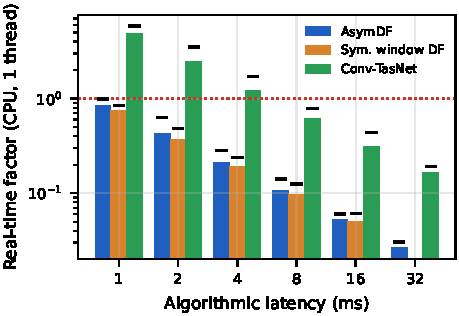
\includegraphics[width=\columnwidth]{figures/rtf.pdf}
\caption{Streaming real-time factor on one CPU thread at batch size one
(bars: median; ticks: p99). Below the red line the model keeps up.}
\label{fig:rtf}
\end{figure}

\subsection{Real-time cost}
Streaming AsymDF takes \ComputestftasymFourms\,ms per chunk regardless of
hop (Fig.~\ref{fig:rtf}), so it keeps up down to 1\,ms latency (RTF
\RtfstftasymOnems\ median, \RtfPstftasymOnems\ p99) on one thread of
\BenchCpu. At 4\,ms it runs at RTF \RtfstftasymFourms, so the delay
heard is about $4 + \ComputestftasymFourms$\,ms. The constant per-chunk
cost shows the time is dominated by per-call framework overhead, not by
arithmetic (\MmacsstftasymFourms\,MMAC/s at 4\,ms). Conv-TasNet's 12 streamed
TCN blocks cost \ComputetasnetFourms\,ms per chunk, so it is
real-time only from 8\,ms upward (RTF \RtftasnetFourms\ at 4\,ms,
\RtftasnetEightms\ at 8\,ms). A fused or compiled kernel would change this
constant, not the algorithmic latency.
